\chapter{深入剖析} 

	如果不理解套接字的具体实现所关联的数据结构和底层协议的工作细节,就很难抓住网络编程的精妙之处,对于TCP套接字(即Socket的实例)来说更是如此。本章就对创建和使用Socket或ServerSocket实例时的底层细节进行了介绍。(本章开始的讨论以及第6.5节同样适用于DatagramSocket和MulticastSocket。而且,由于每个SocketChannel都有一个底层的Socket(其他类型的信道也类似),我们讨论的内容也同样适用于它们。然而,本章大部分内容都针对的是TCP套接字,即,Socket和ServerSocket。)请注意,这些内容仅仅涵盖了一些普通的事件序列,略去了很多细节。尽管如此,我们相信即使是这种基础的理解也是有用的。如果希望了解更详尽内容,可以参考TCP规范[ ],或关于该主题的其他更全面的著作。

	图6.1是一个Socket实例所关联的一些信息的简化视图。JVM和/或其运行的平台(即,主机操作系统中的"套接字层")为这些类的支持提供了底层实现。Java对象上的操作则转换成了在这种底层抽象上的操作。在本章中,"Socket"指的是图6.1中的类之一,而"套接字(socket)"指的是的底层抽象,这种抽象由操作系统提供或由JVM自己实现(例如在嵌入式系统中)。有重要一点需要注意,即运行在统一主机上的其他程序可能也会通过底层套接字抽象来使用网络,因此会与Java Socket实例竞争系统资源,如端口等。

	\clearpage

	\begin{figure}[htbp]%位置选项
		\centering
		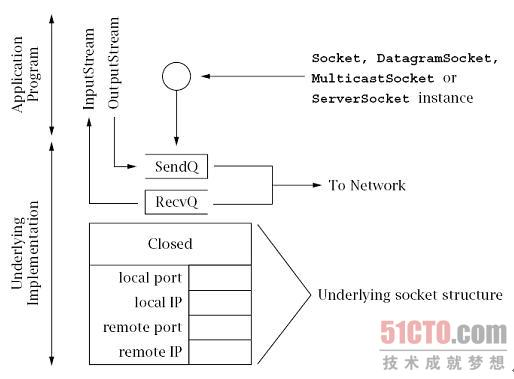
\includegraphics[scale=.6]{img/06.01.jpg}
		\caption{套接字关联的数据结构}
		\label{fig:data.struct.of.socket}
	\end{figure}

	Application Program:应用程序;Underlying Implementation:底层实现;To Network:到网络;Underlying socket structure:底层套接字结构;Socket, DatagramSocket, MulticastSocket or ServerSocket instance:Socket,DatagramSocket,MulticastSocket或ServerSocket实例;

	在此,"套接字结构"是指底层实现(包括JVM和TCP/IP,但通常是后者)的数据结构集,这些数据结构包含了特定Socket实例所关联的信息。例如,套接字结构除其他信息外还包含

	该套接字所关联的本地和远程互联网地址和端口号。本地互联网地址(图中标记为"Local IP")是赋值给本地主机的;本地端口号在Socket实例创建是设置。远程地址和端口号标识了与本地套接字连接的远程套接字(如果有连接的话)。不久,我们将对这些值确定的时间和方式作进一步介绍(第6.5节中有一个简明的概要)。

	一个FIFO(先进先出,First In First Out)队列用于存放接收到的等待分配的数据,以及一个用于存放等待传输的数据的队列。

	对于TCP套接字,还包含了与打开和关闭TCP握手相关的额外协议状态信息。图6.1中,状态是"关闭";所有套接字的起始状态都是关闭的。

	一些多用途操作系统为用户提供了获取底层数据结构"快照"的工具,netstat是其中之一,它在Unix(Linux)和Windows平台上都可用。只要给定适当的选项,netstat就能显示和图6.1中的那些信息:SendQ和RecvQ中的字节数,本地和远程IP地址和端口号,以及连接状态等。netstat的命令行选项有多种,但它的输出看起来是这样的:

	\lstinputlisting[language=Bash,firstline=1,lastline=10]{src/ch06/stp.txt}

	前四行和最后一行描述了正在侦听连接的服务器套接字。(最后一行是一个绑定到IPv6地址的侦听套接字。)第五行代表了到一个Web服务器(80端口)的连接,该服务器已经单方面关闭(见第6.4.2节)。倒数第二两行是现有的TCP连接。如果系统支持的话,你可能想要尝试一下netstat,来测试下文描述的场景的连接状态。然而要知道,这些图中描述的状态转换过程转瞬即逝,可能很难通过netstat提供的"快照"功能将其捕获。

	了解这些数据结构,以及底层协议如何对其进行影响是非常有用的,因为它们控制了各种Socket对象行为的各个方面。例如,由于TCP提供了一种可信赖的字节流服务,任何写入Socket的OutputStream的数据复本都必须保留,直到其在连接的另一端被成功接收。向输出流写数据并不意味着数据实际上已经被发送--它们只是被复制到了本地缓冲区。就算在Socket的OutputStream上进行flush()操作,也不能保证数据能够立即发送到信道。此外,字节流服务的自身属性决定了其无法保留输入流中消息的边界信息。如在第3.3节见到的,这使一些协议的接收和解析过程变得复杂。另一方面,对于DatagramSocket,数据包并没有为重传而进行缓存,任何时候调用send()方法返回后,数据就已经发送给了执行传输任务的网络子系统。如果网络子系统由于某种原因无法处理这些消息,该数据包将毫无提示地被丢弃(不过这种情况很少发生)。

	后面3节对使用TCP字节流服务发送和接收数据的一些微妙之处进行了介绍。然后,第6.4节专注于TCP协议连接的建立和终止。最后,第6.5节讨论了匹配传入的数据包到套接字的过程和绑定端口号的一些规则。

\section{缓冲和TCP}

	作为程序员,在使用TCP套接字时需要记住的最重要一点是:

	不能假设在连接的一端将数据写入输出流和在另一端从输入流读出数据之间有任何一致性。

	尤其是在发送端由单个输出流的write()方法传输的数据,可能会通过另一端的多个输入流的read()方法来获取;而一个read()方法可能会返回多个write()方法传输的数据。

	为了展示这种情况,考虑如下程序:

	\lstinputlisting[language=Java,firstline=15,lastline=28]{src/ch06/stp.txt}

	其中,圆点代表了设置缓冲区数据的代码,但不包含对out.write()方法的调用。在本节的讨论中,"in"代表接收端Socket的InputStream,"out"代表发送端Socket的OutputStream。

	这个TCP连接向接收端传输8000字节。在连接的接收端,这8000字节的分组方式取决于连接两端out.write()方法和in.read()方法的调用时间差,以及提供给in.read()方法的缓冲区大小。

	我们可以认为TCP连接上发送的所有字节序列在某一瞬间被分成了三个FIFO队列:

	1. SendQ:在发送端底层实现中缓存的字节,这些字节已经写入输出流,但还没在接收端主机上成功接收。

	2. RecvQ:在接收端底层实现中缓存的字节,等待分配到接收程序--即从输入流中读取。

	3. Delivered:接收者从输入流已经读取到的字节。

	调用out.write()方法将向SendQ追加字节。TCP协议负责将字节按顺序从SendQ移动到RecvQ。有重要的一点需要明确,这个转移过程无法由用户程序控制或直接观察到,并且在块中(chunks)发生,这些块的大小在一定程度上独立于传递给write()方法的缓冲区大小。

	接收程序从Socket的InputStream读取数据时,字节就从RecvQ移动到Delivered中,而转移的块的大小依赖于RecvQ中的数据量和传递给read()方法缓冲区大小。

	图6.2展示了上例中三次调用out.write()方法后,另一端调用in.read()方法前,以上3个队列的可能状态。不同的阴影效果分别代表了上文中三次调用write()方法传输的不同数据。

	图6.2描述的发送端主机的netstat输出瞬时状态中,会包含类似于以下一行的内容:

	\lstinputlisting[language=Bash,firstline=31,lastline=33]{src/ch06/stp.txt}

	在接收端主机,netstat会显示:

	\lstinputlisting[language=Bash,firstline=35,lastline=37]{src/ch06/stp.txt}

	现在假设接收者调用read()方法时使用的缓冲区数组大小为2000字节,read()调用则将把等待分配队列(RecvQ)中的1500字节全部移动到数组中,返回值为1500。注意,这些数据包括了第一次和第二次调用write()方法时传输的字节。再过一段时间,当TCP连接传完更多数据后,这三部分的状态可能如图6.3所示。

	如果接收者现在调用read()方法时使用4000字节的缓冲区数组,将有很多字节从等待分配队列(RecvQ)转移到已分配队列(Delivered)中。这包括第二次调用write()方法时剩下的1500字节加上第三次调用write()的前2500字节。此时队列的状态如图6.4所示。

	\clearpage

	\begin{figure}[htbp]%位置选项
		\centering
		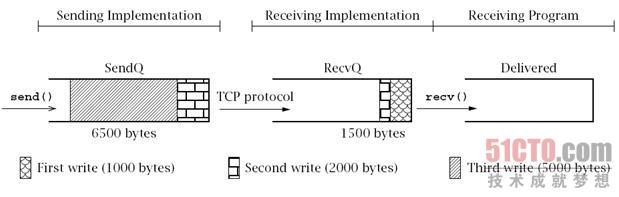
\includegraphics[scale=.6]{img/06.02.jpg}
		\caption{三次调用write()方法后三个队列的状态}
		\label{fig:tree.time.call.write.get.tree.query}
	\end{figure}

	Sending Implementation:发送实现,Receiving Implementation:接收实现,6500 bytes:6500字节,1500 bytes:1500字节,Receiving Program:接收程序,First write(1000 bytes):第一次写操作(1000字节),Second write(2000 bytes):第二次写操作(2000字节),Third write(5000 bytes):第三次写操作(5000字节),TCP protocol:TCP协议

	\clearpage

	\begin{figure}[htbp]%位置选项
		\centering
		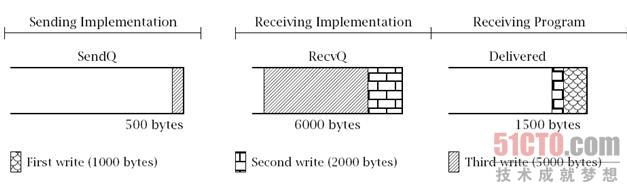
\includegraphics[scale=.6]{img/06.03.jpg}
		\caption{第一次调用read()方法}
		\label{fig:first.time.call.read.func}
	\end{figure}

	Sending Implementation:发送实现,Receiving Implementation:接收实现,500 bytes:500字节,6000 bytes:6000字节,1500 bytes:1500字节,First write(1000 bytes):第一次写操作(1000字节),Second write(2000 bytes):第二次写操作(2000字节),Third write(5000 bytes):第三次写操作(5000字节)

	\clearpage

	\begin{figure}[htbp]%位置选项
		\centering
		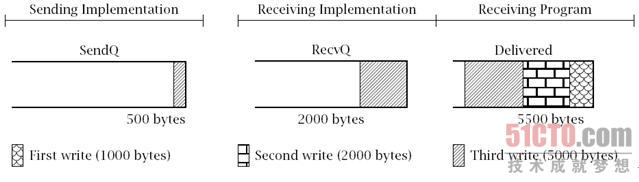
\includegraphics[scale=.6]{img/06.04.jpg}
		\caption{另一次调用read()方法}
		\label{fig:another.call.read.func}
	\end{figure}

	Sending Implementation:发送实现,Receiving Implementation:接收实现,500 bytes:500字节,2000 bytes:2000字节,5500 bytes:5500字节,First write(1000 bytes):第一次写操作(1000字节),Second write(2000 bytes):第二次写操作(2000字节),Third write(5000 bytes):第三次写操作(5000字节)

	下次调用read()方法返回的字节数,取决于缓冲区数组的大小,以及发送方套接字/TCP实现通过网络向接收方实现传输数据的时机。数据从SendQ到RecvQ缓冲区的移动过程对应用程序协议的设计有重要的指导性。我们已经遇到过需要对使用带内(in-band)分隔符成帧(见第3.3节),并通过Socket来接收的消息进行解析的情况。在下面的章节中,我们将考虑另外两个更加微妙的情况。

\section{死锁风险}

	应用程序协议必须设计得非常小心,以避免发生死锁--这种情况下,每个对等端都在阻塞等待其他端完成一些工作。例如,如果在连接建立后,客户端和服务器端都立即尝试接收数据,显然将导致死锁。死锁还可能发生在其他非即时的情况下。

	SendQ和RecvQ缓冲区的容量在具体实现时会受一定的限制。虽然它们使用的实际内存大小会动态地增长和收缩,还是需要有一个硬性的限制,以防止行为异常的程序所控制的单独一个TCP连接将系统的内存全部耗尽。由于这些缓冲区的容量有限,它们可能被填满,事实也的确如此。如果与TCP的流量控制(flow control)机制结合使用,则可能导致另一种形式的死锁。

	一旦RecvQ已满,TCP流控制机制就会产生作用。它将阻止传输发送端主机的SendQ中的任何数据,直到接收者调用输入流的read()方法后腾出了空间。(使用流控制机制的目的是为了保证发送者不会传输太多数据,而超出了接收系统的处理能力。)发送程序可以持续地写出数据,直到SendQ队列被填满,然而,如果在SendQ队列已满时调用out.write()方法,则将阻塞等待,直到有新的空间为止,也就是说直到一些字节传输到了接收到套接字的RecvQ队列中。如果此时RecvQ队列也已经被填满,所有操作都将停止,直到接收程序调用in.read()方法将一些字节传输到了Delivered队列中。

	假设SendQ队列和RecvQ队列的大小分别为SQS和RQS。将一个大小为n的字节数组传递给write()方法调用,其中n > SQS,直到有至少n- SQS字节传递到接收端主机的RecvQ队列后,该方法才会返回。如果n的大小超过了(SQS + RQS),write()方法则将在接收程序从输入流读取了至少n? (SQS + RQS)字节后才会返回。如果接收程序没有调用read()方法,大数据量的send()调用则无法成功。特别是当连接的两端同时分别调用它们输出流的write()方法,而它们的缓冲区大小又大于SQS + RQS时,将发生死锁:两个write操作都不能完成,两个程序都将永远保持阻塞状态。

	下面考虑一个具体的例子,即主机A上的程序和主机B上的程序之间的一个连接。假设A和B上的SQS和RQS都是500字节,图6.5展示了两个程序试图同时发送1500字节时的情况。主机A上的程序中的前500字节已经传输到了另一端,另外500字节已经复制到了主机A的SendQ队列中,余下的500字节则无法发送(因此out.write()方法将无法返回)直到主机B上的RecvQ队列有空间空出来。然而不幸的是主机B上的程序也遇到了同样的情况。因此两个程序的write()方法调用都永远无法完成。

	\clearpage

	\begin{figure}[htbp]%位置选项
		\centering
		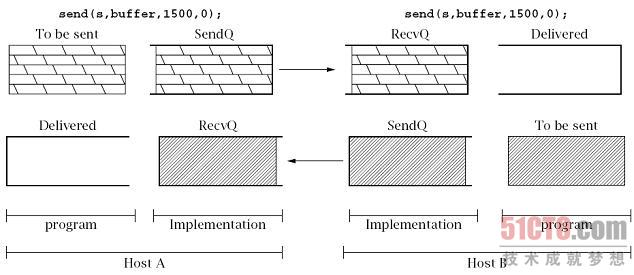
\includegraphics[scale=.6]{img/06.05.jpg}
		\caption{由于连接两端同时调用输出流的write()方法而导致了死锁}
		\label{fig:dead.lock.by.call.both.side}
	\end{figure}

	program:程序,Implementation:具体实现, To be sent:即将发送

	这个故事的寓意:要仔细设计协议,以避免在两个方向上传输大量数据时产生死锁。

	这种情况真的会发生吗?让我们回顾一下第4.5节中的压缩协议示例。尝试运行该压缩客户端并传递给它一个大文件,该文件压缩后仍然很大。在此,"大"的精确定义取决于你的系统,不过压缩后依然超过2MB的文件应该就可以了。每次read/write操作,压缩客户端都向控制台打印一个"R"或"W"。如果该文件的未压缩版本和压缩版本都足够大,你的客户端将在打印出一堆W后停止,并且不会打印任何R,程序也不过终止。

	为什么会发生这种情况呢?程序CompressClient.java在尝试从压缩流读取数据前,先要将所有未压缩的数据发送到压缩服务器。而另一方面,服务器只是简单地读取未压缩字节序列,并将压缩后的序列返回给客户端。(服务器在写回压缩数据前,其读取的字节数取决于所使用的压缩算法。)考虑这种情况:客户端和服务器端的SendQ队列和RecvQ队列中都有500字节的数据,而客户端发送了一个大小为10000字节(未压缩)的文件。同时假设对于这个文件,服务器读取1000字节并返回500字节,即压缩比为2:1。当客户端发送了2000字节后,服务器端将最终全部读取这些字节,并发回1000字节,此时客户端的RecvQ队列和服务器端的SendQ队列都将被填满。当客户端又发送了1000字节并且被服务器端全部读取后,服务器端后续的任何write操作尝试都将阻塞。当客户端又发送了另外1000字节后,客户端的SendQ队列和服务器端的RecvQ队列都将填满。后续的客户端write操作将阻塞,从而形成死锁。

	\lstinputlisting[language=Java,firstline=1]{src/ch06/CompressClient.java}

	如何解决这个问题?方案之一是在不同的线程中执行客户端的write循环和read循环。一个线程从文件中反复读取未压缩的字节并将其发送给服务器,直到到底文件的结尾,然后调用该套接字的shutdownOutput()方法。另一个线程从连接到服务器的输入流中反复读取压缩后的字节,并将其写入输出文件,直到到达了输入流的结尾(即服务器关闭了套接字)。如果一个线程阻塞了,另一个线程仍然可以独立执行。要实现这个功能,我们可以对客户端代码进行简单的修改,像下面这样将CompressClient.java中的SendBytes()方法调用放到一个线程中:

	\lstinputlisting[language=Java,firstline=41,lastline=48]{src/ch06/stp.txt}

	CompressClientNoDeadlock.java的完整版本请参见本书的网站。

	\lstinputlisting[language=Java,firstline=1]{src/ch06/CompressClientNoDeadlock.java}

	当然,解决这个问题也可以不使用多线程,而是使用第5章介绍的非阻塞Channel和Selector。

\section{性能相关}

	在TCP实现中,将用户数据复制到SendQ队列中不仅是因为可能重传数据,这还与性能有关。尤其是SendQ和RecvQ缓冲队列的大小,会对TCP连接的数据吞吐量产生影响。吞吐量是指用户数据字节从发送端发送到接收程序的频率。在要传输大量数据的程序中,我们希望能够最大化这个频率。在没有网络容量或其他限制的情况下,越大的缓冲区通常能够实现越高的吞吐量。

	这种情况发生的原因,与底层实现中将数据从缓冲区中存取时的系统耗费有关。如果要传输n字节的数据,使用大小为n的缓冲区调用一次write()方法,通常要比使用大小为1字节的缓冲区调用n次write()方法效率要高很多。[ ] 然而,如果调用write()方法时使用了比SQS(SendQ队列的大小)大很多的缓冲区,系统还需要将数据从用户地址转换为大小为SQS的块(chunks)。也就是说,套接字底层实现先将SendQ队列缓冲区填满,等待TCP协议将数据转移出去,再重新填满SendQ队列缓冲区,再等待数据转移,反复进行。套接字底层实现每次都要等待数据从SendQ队列中移出,这就以系统耗费的形式(系统需要进行上下文切换)浪费了一些时间。这种系统耗费与重新调用一次write()方法的情况相似。因此,调用write()方法时的实际有效缓冲区大小要受SQS的限制。从InputStream读取数据也是一样的道理:即使提供给read()方法的缓冲区很大,数据还是会被复制成RQS大小的块,在块之间又会产生新的系统耗费。

	如果程序的数据吞吐量是一个重要的性能参数,你可能希望通过Socket的setSendBufferSize()和setReceiveBufferSize()方法来改变发送和接收缓冲区的大小。虽然每个缓冲区都有系统指定的最大容量,但是在现代系统上缓冲区的容量通常要比系统的默认大小要大很多。要记住一点,只有当程序要一次发送比缓冲区容量大很多的数据时才需要考虑这些情况。同时还有注意,如果处理了一些从Socket的基本输入流继承而来的更高层次的流(例如,使用它来创建一个FilterOutputStream实例或PrintWriter实例),这些因素产生的效果就会略有不同,因为更高层次的流可能会执行它们字节的内部缓存或增加额外的系统开销。


	\subsection{TCP套接字的生存周期}

		新的Socket实例创建后(无论是通过公有的构造函数,或是通过调用ServerSocket类的accept()方法)立即就能用于发送和接收数据。也就是说,当Socket实例返回时,它已经连接到了一个远程终端,并通过协议的底层实现完成了TCP消息或握手信息的交换。

		下面,让我们进一步详细考虑底层的数据结构如何到达已连接或"已建立(Established)"状态。后面你将看到,这些细节会对可靠性的定义和创建一个绑定到特定端口的Socket或ServerSocket的能力产生影响。

		\subsection{连接}

		Socket构造函数的调用与客户端连接建立时所关联的协议事件之间的关系如图6.6所示。在本节所有的示意图中,大箭头都表示导致底层套接字数据结构发生状态改变的外部事件。在应用程序中发生的事件(即方法调用和返回)显示在图个上部;如消息到达等事件显示在图的下部。所有图的时间顺序都是从左到右的;客户端的互联网地址表示为A.B.C.D,服务器端的互联网地址表示为W.X.Y.Z; 服务器的端口号是Q。(我们描述的是IPv4地址,不过这里介绍的内容都适用于IPv4和IPv6。)

		当客户端以服务器端的互联网地址W.X.Y.Z和端口号Q作为参数,调用Socket的构造函数时,底层实现将创建一个套接字实例,该实例的初始状态是关闭状态(Closed)。如果在调用构造函数时客户端没有指定本地地址或端口号,底层实现将选择一个没有被其他TCP套接字使用的本地端口号(P)。同时还要指定本地的互联网地址,如果没有显式地指定,则将向服务器发送数据报文的网络接口地址作为本地地址。底层实现将本地和远程地址和端口复制到底层套接字的数据结构,并初始化TCP连接建立时的握手消息。

		\clearpage

		\begin{figure}[htbp]%位置选项
			\centering
			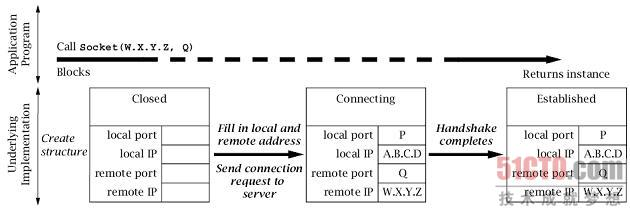
\includegraphics[scale=.6]{img/06.06.jpg}
			\caption{客户端连接建立}
			\label{fig:client.create.connection}
		\end{figure}

		Application Program:应用程序,Underlying Implementation:底层实现,Call Socket(W.X.Y.Z,Q):调用Socket(W.X.Y.Z,Q),Blocks:阻塞等待,Create structure:创建数据结构,local port:本地端口,local IP:本地IP地址,remote port:远程端口号,remote IP:远程IP地址,Fill in local and remote address:填入本地和远程地址,Send connection request to server:向服务器发送连接请求,Handshake completes:握手消息完成,Returns instance:返回实例,Connecting:正在连接,Established:连接建立完成

		TCP的开放握手也称为3次握手(3-way handshake),因为这通常包括3条消息:一条从客户端到服务器端的连接请求,一条从服务器端到客户端的确认消息,以及另一条从客户端到服务器端的确认消息。客户端一收到服务器端发来的确认消息,就立即认为连接已经成功建立。通常情况这个过程发生得很快。然而,互联网是一种尽力而为(best-effort)的网络,客户端的起始消息或服务器端的回复消息都可能在传输过程中丢失。出于这个原因,TCP协议实现将以递增的时间间隔重复发送几次握手消息。如果TCP客户端在一段时间后还没有收到服务器的回复消息,则发生超时并放弃连接。这种情况下,构造函数将抛出IOException异常。连接的超时通常比较长,因此要经过几分种的时间Socket的构造函数才会失败。

		在初始的握手消息发送之后,并在接收到服务器端的回复消息之前(即图6.6的中间部分),客户端主机上netstat的输出将类似于以下内容:

		\lstinputlisting[language=Java,firstline=51,lastline=53]{src/ch06/stp.txt}

		其中,"\verb|SYN_SENT|"是在第一条和第二条握手消息之间,客户端状态的专业名称。

		如果服务器并没有接收连接(比如,目标地址的给定端口上没有关联任何程序),服务器端的TCP将发送一条拒绝消息而不是确认消息,并且构造函数几乎立即会抛出一个IOException异常。否则,在客户端收到了服务器端的肯定回复后,其netstat的输出将类似于以下内容:

		\lstinputlisting[language=Java,firstline=56,lastline=58]{src/ch06/stp.txt}

		服务器端的事件序列则有所不同,我们在图6.7,6.8和6.9中对其进行描述。服务器首先创建一个ServerSocket实例,并将其与已知端口相关联(在此为Q)。套接字实现为新的ServerSocket实例创建了一个底层数据结构,并将Q赋给本地端口,将特定的通配符地址(图中的"*")赋给本地IP地址。(服务器也可能会在构造函数中指定一个本地IP地址,但是通常不这样做。对于服务器主机有多个IP地址的情况,不指定本地地址使套接能够接受发送到该服务器主机任何地址的连接请求。)套接字的状态设置为"LISTENING",指示该套接已经准备好接受传入该端口的连接请求。图6.7描述了这个过程。服务器端netstat的输出中会包含类似于如下一行的内容:

		\lstinputlisting[language=Java,firstline=61,lastline=63]{src/ch06/stp.txt}

		\clearpage

		\begin{figure}[htbp]%位置选项
			\centering
			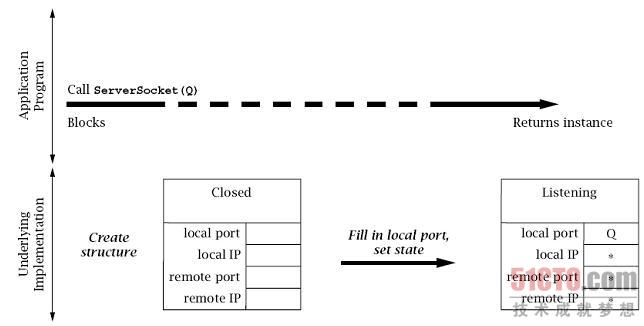
\includegraphics[scale=.6]{img/06.07.jpg}
			\caption{服务器端套接字设置}
			\label{fig:server.create.socket}
		\end{figure}

		Application Program:应用程序;Underlying Implementation:底层实现;Call ServerSocket(Q):调用ServerSocket(Q);Blocks:阻塞等待;Returns instance:返回实例;Create structure:创建数据结构;Closed:关闭;Listening:侦听;local port:本地端口;local IP:本地IP地址;remote port:远程端口号;remote IP:远程IP地址;Fill in local port,set stat:填入本地端口号,设置状态;

		现在服务器可以调用ServerSocket的accept()方法,该方法将阻塞等待,直到与某个客户端完成了开放握手信息交换,并成功建立了新的连接。因此我们关注于(见图6.8)当客户端连接请求到来时,TCP实现中发生的事件。注意,该图中描述的内容全都隐蔽地发生在TCP底层实现中。

		当客户端的连接请求到来时,将为该连接创建一个新的套接字数据结构。新套接字的地址根据到来的分组报文设置:分组报文的目标互联网地址和端口号(分别为W.X.Y.Z和Q)成为该套接字的本地互联网地址和端口号;而分组报文的源地址和端口号(分别为A.B.C.D和P)则成为该套接字的远程互联网地址和端口号。注意,新套接字的本地端口号总是与ServerSocket的端口号一致。新套接字的状态设置为指示"正在连接(Connecting)"(在服务器方,专业术语称其为\verb|SYN_RCVD|),并将其添加到ServerSocket套接字数据结构所关联的一个未完全连接的套接字列表中。注意,ServerSocket自己并不改变状态,其地址信息也不会有任何改变。此时,netstat的输出内容应该包括原始的侦听套接字和新创建的套接字:

		\lstinputlisting[language=Java,firstline=65,lastline=68]{src/ch06/stp.txt}

		除了要创建一个新的底层套接字数据结构外,服务器方的TCP实现还要向客户端发回一个TCP握手确认消息。

		\clearpage

		\begin{figure}[htbp]%位置选项
			\centering
			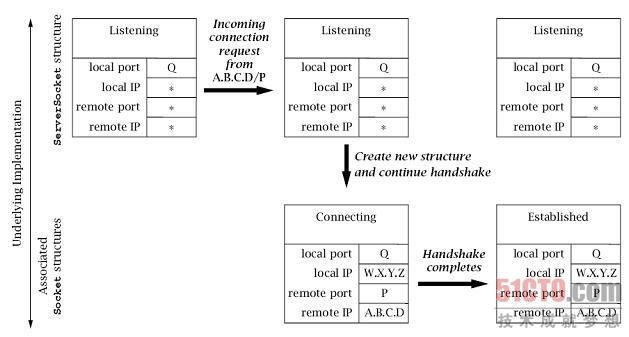
\includegraphics[scale=.6]{img/06.08.jpg}
			\caption{处理传入的连接请求}
			\label{fig:deal.income.connect.req}
		\end{figure}

		Underlying Implementation:底层实现;Associated Socket structures:关联的Socket数据结构;ServerSocket structure:ServerSocket数据结构;local port:本地端口;local IP:本地IP地址;remote port:远程端口号;remote IP:远程IP地址;Listening:侦听;Connecting:正在连接;Established:连接建立;Incoming connection request from A.B.C.D/P:从A.B.C.D/P传来的连接请求;Create new structure and continue handshake:创建新的数据结构并继续握手;Handshake completes:握手完成。

		然而,在接收到客户端发来的3次握手的第3条消息之前,服务器端TCP并不会认为握手消息已经完成。第3条握手消息到来后,新数据结构的状态则设置为"ESTABLISHED",并将其移动到ServerSocket数据结构关联的另一个套接字数据结构列表中,该列表代表了能够通过ServerSocket的accept()方法进行接收的已成功建立连接。(如果第3条握手消息接收失败,最终会将"Connecting"状态的数据结构删除。)此时netstat的输出将包含:

		\lstinputlisting[language=Java,firstline=71,lastline=74]{src/ch06/stp.txt}

		现在,我们来考虑(见图6.9)服务器程序调用了ServerSocket的accept()方法后发生的事情。只要其关联的套接字数据结构列表中有新的连接到来,该方法调用就立即停止阻塞。(注意,在调用accept()方法时,这个列表可能已经是非空状态。)此时,一个新的连接数据结构将从列表中移除,并为其创建一个Socket实例,作为accept()方法的返回值。

		有非常重要的一点需要注意,在ServerSocket关联的列表中的每个数据结构,都代表了一个与另一端的客户端已经完成建立的TCP连接。实际上,客户端只要接收到了开放握手的第2条消息,就可以立即发送数据--这可能比服务器调用accept()方法为其获取一个Socket实例要早很长时间。

		\clearpage

		\begin{figure}[htbp]%位置选项
			\centering
			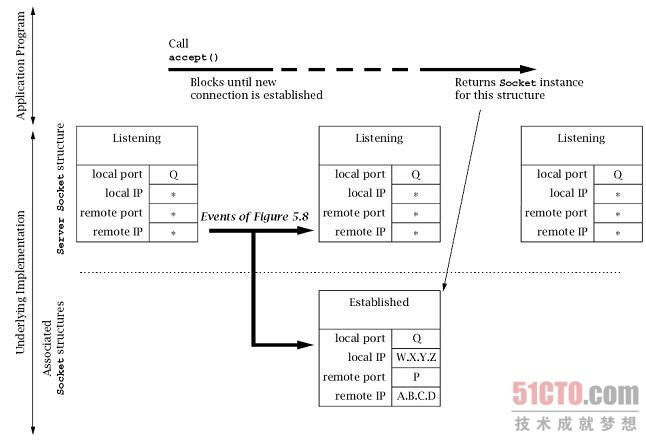
\includegraphics[scale=.6]{img/06.09.jpg}
			\caption{accept()处理}
			\label{fig:accept.process}
		\end{figure}

		Application Program:应用程序;Underlying Implementation:底层实现;Associated Socket structures:关联的Socket数据结构;ServerSocket structure:ServerSocket数据结构;Call accept():调用accept()方法;Blocks until new connection is established:阻塞等待,直到建立了新的连接;Return Socket instance for this structure:为此数据结构返回Socket实例;local port:本地端口;local IP:本地IP地址;remote port:远程端口号;remote IP:远程IP地址;Events of Figure 5.8:图5.8中的事件;Listening:侦听;Established:连接建立。

	\subsection{关闭TCP连接}

		TCP协议有一个优雅的关闭(graceful close)机制,以保证应用程序在关闭连接时不必担心正在传输的数据会丢失。如第4.5节的压缩示例程序所示,这个机制还设计为允许两个方向的数据传输相互独立地终止。关闭机制的工作流程是:应用程序通过调用连接套接字的close()方法或shutdownOutput()方法表明数据已经发送完毕。此刻,底层的TCP实现首先将留存在SendQ队列中的数据传输出去(还要依赖于另一端RecvQ队列的剩余空间),然后向另一端发送一个关闭TCP连接的握手消息。该关闭握手消息可以看作是流终止标志:它告诉接收端TCP不会再有新的数据传入RecvQ队列了。(注意,关闭握手消息本身并没有传递给接收端应用程序,而是通过read()方法返回-1来指示其在字节流中的位置。)正在关闭的TCP将等待其关闭握手消息的确认信息,该确认信息表明在连接上传输的所有数据已经安全地传输到了RecvQ中。只要收到了确认消息,该连接就变成"半关闭(Half closed)"状态。直到连接的另一个方向上收到了对称的握手消息后,连接才完全关闭--也就是说,连接的两端都表明它们再没有数据要发送了。

		TCP连接的关闭事件序列可能以两种方式发生:一种方式是先由一个应用程序调用close()方法(或shutdownOutput()方法),并在另一端调用close()方法之前完成其关闭握手消息;另一种方式是两端同时调用close()方法,它们的关闭握手消息在网络上交叉传输。图6.10展示了以第一种方式关闭连接时,底层实现中的事件序列。关闭握手消息已经发送,套接字数据结构的状态也已经设置为"Closing"(专业术语称为"\verb|FIN_WAIT_1|"),然后close()调用返回。完成这些工作后,将禁止在该Socket上的任何读写操作(会抛出异常)。当收到关闭握手确认消息后,套接字数据结构的状态则改变为"半关闭"(专业术语称为"\verb|FIN_WAIT_2|"),这种状态将一直持续,直到接收到另一端的关闭握手消息。此时,客户端netstat的输出内容将展示连接的状态为:

		\lstinputlisting[language=Java,firstline=77,lastline=79]{src/ch06/stp.txt}

		(在首先发起关闭的主机上,\verb|FIN_WAIT_2|是"半关闭"状态的专业术语。图中由"Closing"指示的状态的专业术语是\verb|FIN_WAIT_1|,不过该状态非常转瞬即逝,很难被netstat捕获到。)

		注意,如果连接处于半关闭状态时,远程终端已经离开,那么本地底层数据结构则将无限期地保持在该状态。当另一端的关闭握手消息到达后,则发回一条确认消息并将状态改变成"Time-Wait"。虽然应用程序中相应的Socket实例可能早已消失,与


		\clearpage

		\begin{figure}[htbp]%位置选项
			\centering
			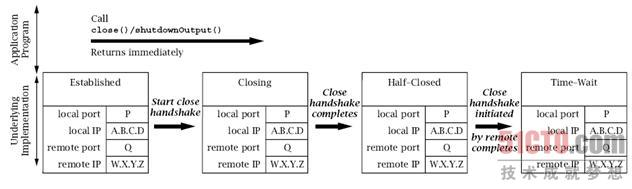
\includegraphics[scale=.6]{img/06.10.jpg}
			\caption{首先关闭一端的TCP连接}
			\label{fig:close.one.side.tcp}
		\end{figure}

		Application Program:应用程序;Underlying Implementation:底层实现;Call close()/shutdownOutput():调用close()/shutdownOutput()方法;Returns immediately:立即返回;Start close handshake:开始关闭握手;Close handshake completes:关闭握手完成;Close handshake initiated by remote completes:由远端发起的关闭握手完成;local port:本地端口;local IP:本地IP地址;remote port:远程端口号;remote IP:远程IP地址;

		在图6.10的右端时,netstat的输出内容包括:

		\lstinputlisting[language=Java,firstline=81,lastline=83]{src/ch06/stp.txt}

		图6.11简单展示了没有首先发起关闭的终端上的事件序列。关闭握手消息到达后,它立即发回一个确认消息,并将连接状态改变为"Close-Wait"。该主机上netstat的输出内容显示:

		\lstinputlisting[language=Java,firstline=85,lastline=87]{src/ch06/stp.txt}

		此时,只需要等待应用程序调用Socket的close()方法。调用该方法后,将发起最终的关闭握手消息,并释放底层套接字数据结构,虽然对原始Socket实例的引用仍然留存在Java程序中。

		注意这样一个事实:close()方法和shutdownOutput()方法都没有等待关闭握手的完成,而是调用后立即返回。你可能会问,发送者怎样能保证已发送的数据能够真正到底接收程序呢(即Delivered)?实际上,当应用程序调用close()或shutdownOutput()方法并成功关闭连接时,的确可能还有数据留存在SendQ队列中。如果连接的任何一端在数据传输到RecvQ队列之前崩溃,数据将丢失,而发送端应用程序却不会知道。

		最好的解决方案是设计一种应用程序协议,以使首先调用close()方法的一方在接收到了应用程序层的数据已接收保证后,才真正执行关闭操作。例如,当我们的TCPEchoClient程序接收到了它所发送的数据的完全拷贝后,它就能够知道此时在连接两个方向上都没有数据在传输,因此可以安全地关闭连接。


		\clearpage

		\begin{figure}[htbp]%位置选项
			\centering
			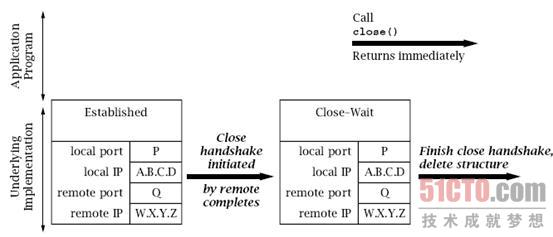
\includegraphics[scale=.6]{img/06.11.jpg}
			\caption{在另一端关闭后关闭TCP连接}
			\label{fig:close.other.side.side.tcp}
		\end{figure}

		Application Program:应用程序;Underlying Implementation:底层实现;Call close():调用close()方法;Return immediately:立即返回;Close handshake initiated by remote completes:远端发起的关闭握手完成;Finish close handshake, delete structure:完成关闭握手,删除数据结构;local port:本地端口;local IP:本地IP地址;remote port:远程端口号;remote IP:远程IP地址;

		Java的确提供了一种能够修改Socket的close()的行为的方法,即setSoLinger()方法。setSoLinger()用于控制close()方法在返回前是否等待关闭握手的完成。它有两个参数:一个布尔变量用来指示是否等待;一个整型变量用来指定放弃之前等待的时间(单位为秒)。也就是说,使用setSoLinger()设置了超时时间后,close()方法将阻塞等待,直到关闭握手完成或指定时间超时。然而,在本书的写作期间,即使在setSoLinger()设置的时间限制已经超过时,close()方法也没有提供任何信息来指示关闭握手的失败。换句话说,setSoLinger()方法没有为当前实现的应用程序提供任何额外担保。

		关闭TCP连接的最后微妙之处在于对Time-Wait状态的需要。TCP规范要求在终止连接时,两端的关闭握手都完成后,至少要有一个套接字在Time-Wait状态保持一段时间。这个要求的提出是由于消息在网络中传输时可能延迟。如果在连接两端都完成了关闭握手后,它们都移除了其底层数据结构,而此时在同样一对套接字地址之间又立即建立了新的连接,那么前一个连接在网络上传输时延迟的消息就可能在新连接建立后到达。由于其包含了相同的源地址和目的地址,旧消息就会被错误地认为是属于新连接的,其包含的数据就可能被错误地分配到应用程序中。

		虽然这种情形可能很少发生,TCP还是使用了包括Time-Wait状态在内的多种机制对其进行防范。Time-Wait状态用于保证每个TCP连接都在一段平静时间内结束,这期间不会有数据发送。平静时间的长度应该等于分组报文在网络上存留的最长时间的两倍。因此,当一个连接完全结束(即套接字数据结构离开Time-Wait状态并被删除),并为同样一对地址上的新连接清理道路后,就不会再有旧实例发送的消息还存留在网络中。实际上,平静时间的长度要依赖于具体实现,因为没有机制能真正限制分组报文在网络上能够延迟的时间。通常使用的时间范围是4分钟减到30秒,或更短。

		Time-Wait状态最重要的作用是,只要底层套接字数据结构还存在,就不允许在相同的本地端口上关联其他套接字。尤其是试图使用该端口创建新的Socket实例时,将抛出IOException异常。

\section{解调多路复用揭秘}

	在前面的讨论中已经隐含表明一个事实,即同一个机器上的不同套接字可以有相同的本地地址和端口号。例如,在只有一个IP地址的机器上,每个通过ServerSocket的accept()方法接收的新Socket实例都将使用与ServerSocket相同的本地端口号。显然,要确定传入的分组报文应该分配到那个套接字(即,解调多路复用)不仅仅是查看分组报文的目的地址和端口。


		\clearpage

	\begin{figure}[htbp]%位置选项
		\centering
		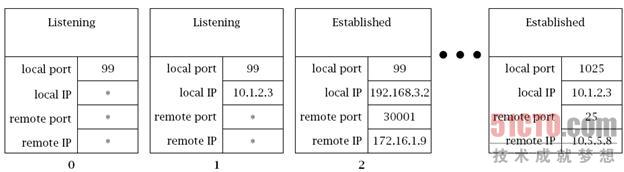
\includegraphics[scale=.6]{img/06.12.jpg}
		\caption{匹配了多个套接字的解调多路复用}
		\label{fig:match.muti.socket.ru}
	\end{figure}

	local port:本地端口;local IP:本地IP地址;remote port:远程端口号;remote IP:远程IP地址;

	否则传入的分组报文应该分配给哪个套接字就会含糊不清。对于TCP和UDP来说,将传入的分组报文匹配到某个套接字的过程是一样的,可以归纳为以下几点:

	套接字数据结构中的本地端口号必须与传入的分组报文的目的端口号相匹配。

	在套接字数据结构中,任何包含了通配符(*)的字段可以匹配分组报文中相应字段的任何值。

	如果有一个以上的套接字数据结构与传入的分组报文地址的四个字段匹配,那么谁使用的通配符少,谁就获得该分组报文。

	例如,考虑一个主机有两个IP地址的情况,10.1.2.3和192.168.3.2,还有如图6.12所示的活跃的TCP套接字数据结构子集。标记为0的数据结构与一个ServerSocket关联,有一个通配符本地地址,端口号为99。标记为1的套接字数据结构也关联了同一个端口号的ServerSocket,但其本地地址指定为10.1.2.3(因此它只接收发向这个地址的连接请求)。数据结构2代表了通过ServerSocket为数据结构0接收的一个连接,因此有相同的本地端口号,但也填入了本地和远程互联网地址。其他套接字则属于其他活跃的连接。现在考虑一个分组报文,其源IP地址是172.16.1.10,源端口号是56789,目的IP地址是10.1.2.3,目的端口号是99。该报文将分配到与数据结构1相关联的套接字上,因为该套接字匹配的通配符最少。

	当程序试图使用特定的本地端口号创建套接字时,要检查已有的套接字以确保没有其他套接字已经使用了那个本地端口。如果已经有套接字与构造函数中指定的本地端口和本地IP地址(如果有的话)相匹配,Socket的构造函数将抛出一个异常。这在如下情形中将导致一些问题:

	1.客户端程序用特定的本地端口号P创建了一个Socket实例,并通过它与服务器进行通信。

	2.客户端关闭了Socket,底层数据结构进入了Time-Wait状态。

	3.客户端程序终止后又立即重新启动。

	如果新的客户端化身试图使用同样的本地端口号,而由于其他数据结构正处于Time-Wait状态,Socket构造函数将抛出IOException异常。在写本书期间,解决这个问题的唯一途径是等待底层数据结构离开Time-Wait状态。

	那么怎么确定本地或远程的地址和端口号呢?对于ServerSocket,所有构造函数都要求传入本地端口号。本地地址可能会在构造函数中指定,否则,就使用通配符(*)地址。ServerSocket的远程地址和端口号始终是通配符。对于Socket,所有构造函数都要求传入特定的远程地址和端口号。本地地址或端口号可能会在构造函数中指定,否则,本地地址就使用用来建立到服务器的连接的网络接口地址,本地端口号就随机选择一个大于1023的未使用端口号。对于accept()方法返回的Socket实例,本地地址是从客户端发起的初始握手消息的目的地址,本地端口号是SeverSocket的本地端口,远程地址和端口号则是客户端的本地地址和端口号。对于DatagramSocket,本地地址和端口可能会在构造函数中指定,否则,本地地址将使用通配符地址,本地端口则随机选择一个大于1023的未使用端口号,远程地址和端口号都初始化为通配符并一直保持下去,除非调用connect()方法指定了特定的值。

